\subsubsection{Data collection process}
The Mapbox Static Images API was used to retrieve all the satellite images used in this project.

Initially, a training set of 250 satellite images was collected to train the Yolo model.

Our project has two main Python scripts, \texttt{parking\_detection.py} and \texttt{parking\_detection\_local.py} to localize parking spots.
In \texttt{parking\_detection.py}, the satellite images (Mapbox Satellite) and corresponding road mask images (Mapbox Streets) are retrieved for a specific area contained within a bounding box, defined by its top-left and bottom-right coordinates, directly from the Mapbox API.
From the coordinates of the specific bounding box, the center coordinates of all the images necessary to make up that area are calculated, and the images are then retrieved.
While in \texttt{parking\_detection\_local.py}, the original parking detection script is adapted to run on a database of locally stored Mapbox Satellite images and the corresponding Mapbox Streets images, covering the entirety of Dublin city.

Extensive testing was done at all the different stages of development of the scripts to identify the optimal thresholds and parameters using test images from Mapbox, in a variety of scenarios including edge cases or cases prone to causing issues.

\subsubsection{YOLO model used for car detection}
YOLO (You Only Look Once) is an object detection and image segmentation model launched in 2015 which quickly gained popularity for its high speed and accuracy compared to models of the time like \fcolorbox{yellow}{yellow}{find reference.}\\
We started playing with this model because on label studio there was an option to automate the labelling using an integration of the YOLOv5 model. However, this integration was not working which caused us to dig further into Ultralytics, the company behind the YOLO models.\\ \\
Several papers focusing on object detection cited YOLO over other popular models such as \fcolorbox{yellow}{yellow}{find the reference}. A key challenge that influences the choice of model for the object detection task is effectively managing fluctuations in image resolutions and aspect ratios, as well as the computational resources required to run image detection models.\\

There are two main types of models for object detection tasks: single stage and two-stage. The figure below from \cite{singlevstwodetectorimg} illustrates the process for both.
%single vs two stage model process
\begin{figure}[h!]
  \centering
  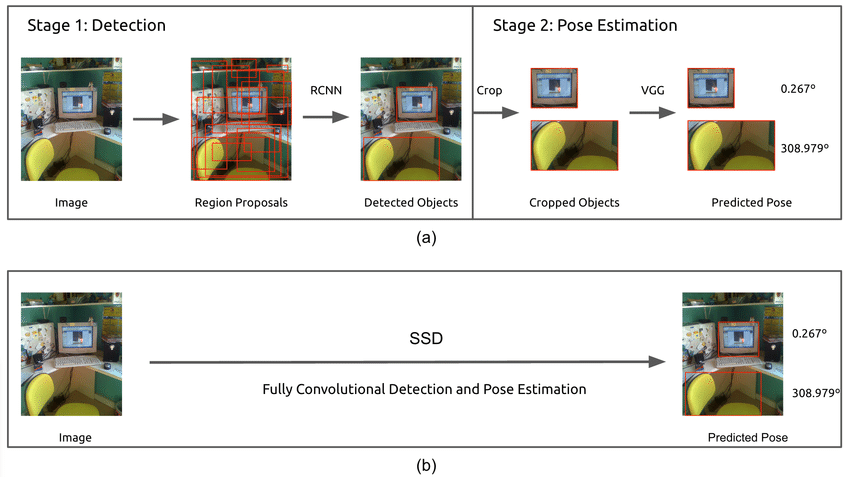
\includegraphics[width=0.7\textwidth]{images/single-vs-two-stage-obj-detector.png}
  \caption{Single vs Two-Stage Object Detection Process}
\end{figure}
\textbf{Single stage} object detector models processes an image through a feature extractor using a CNN (Convolutional Neural Network) and then directly uses the extracted features for classification and regression of bounding boxes. These models are very fast which is why they are popular for real-time object detection tasks; however their accuracy performance can sometimes be poor. Examples of single stage models are SSD, YOLO and RefineDet (\cite{yoloversionsliterature}.)\\
\textbf{Two stage} object detector models divides the process into two main steps. First, it extracts features from the image using a CNN, then selects regions of interests that will only be used for classification and regression of bounding boxes. These models are much more accurate than one stage detectors and are used for tasks where accuracy is prioritized over speed in the medical field for example RCNN, Fast-RCNN and Faster-RCNN(\cite{singlevstwostagedetectors}).\\

For the scope of this project, we chose to continue with the YOLO models because of their speed, their scalability, their lack of computational resources and they are free!\\

We moved away from Label studio and studied the Ultralytics documentation and tried out the YOLOv5 model to recognise the cars on the satellite images. We experimented with different versions of the YOLOv5 model, then slowly levelled up the versions up to version 8, monitoring metrics such as mAP (Mean Average Precision), F1-score and the false positive rate. The figure below shows the metrics of the model as we iteratively experimented up the version chain.
%model metrics graph
\begin{figure}[h!]
  \centering
  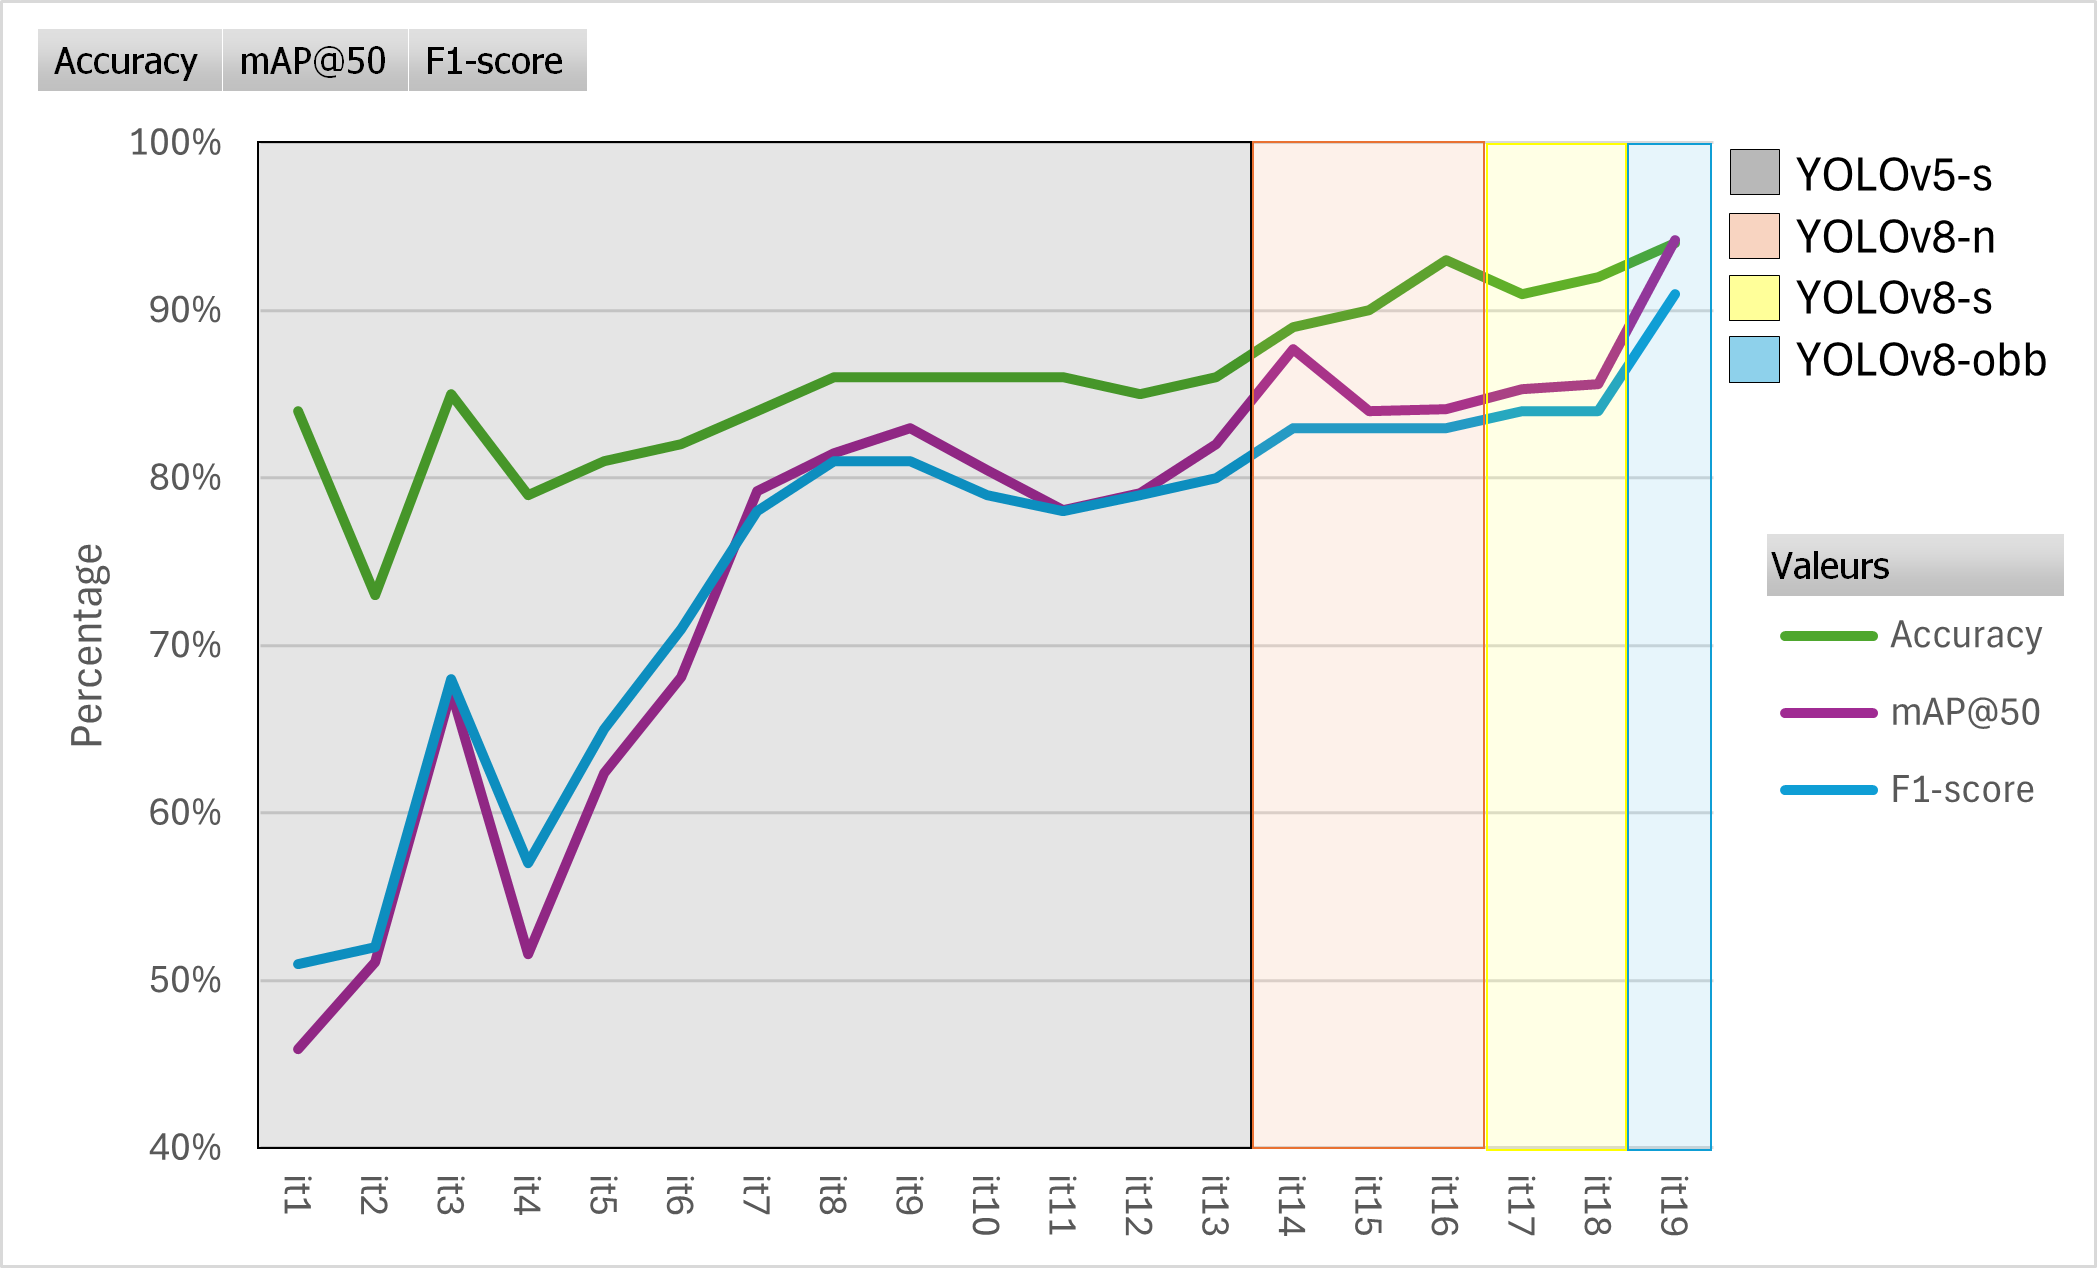
\includegraphics[width=0.85\textwidth]{images/yolo-results.png}
  \caption{YOLO Model training graph}
\end{figure}
We ended the object detection modelling training with the YOLOv8 - Oriented Bounding Boxes (OBB). The YOLOv8 model has been pre-trained on the COCO (Common Object in Context) dataset, a popular large scale dataset with 200,000 images across 80 object categories commonly used for benchmarking computer vision models (\cite{cocodataset}).\\
Oriented bounding boxes are a newer type of bounding box where the bounding box capture the orientation of the object providing a more accurate fit of the object. They are defined by 5 parameters (center xy, width, height and rotation angle) and capture the object's spatial orientation more precisely, reducing overlap and improving the robustness of the object detection model (\cite{obblit}).\\
Below you can see the difference in bounding boxes between the labelled image used for the non-OBB YOLOv5 \& YOLOv8 iterations versus the OBB YOLOv8.
%obb vs non obb bounding boxes
\begin{figure}[h!]
  \centering
  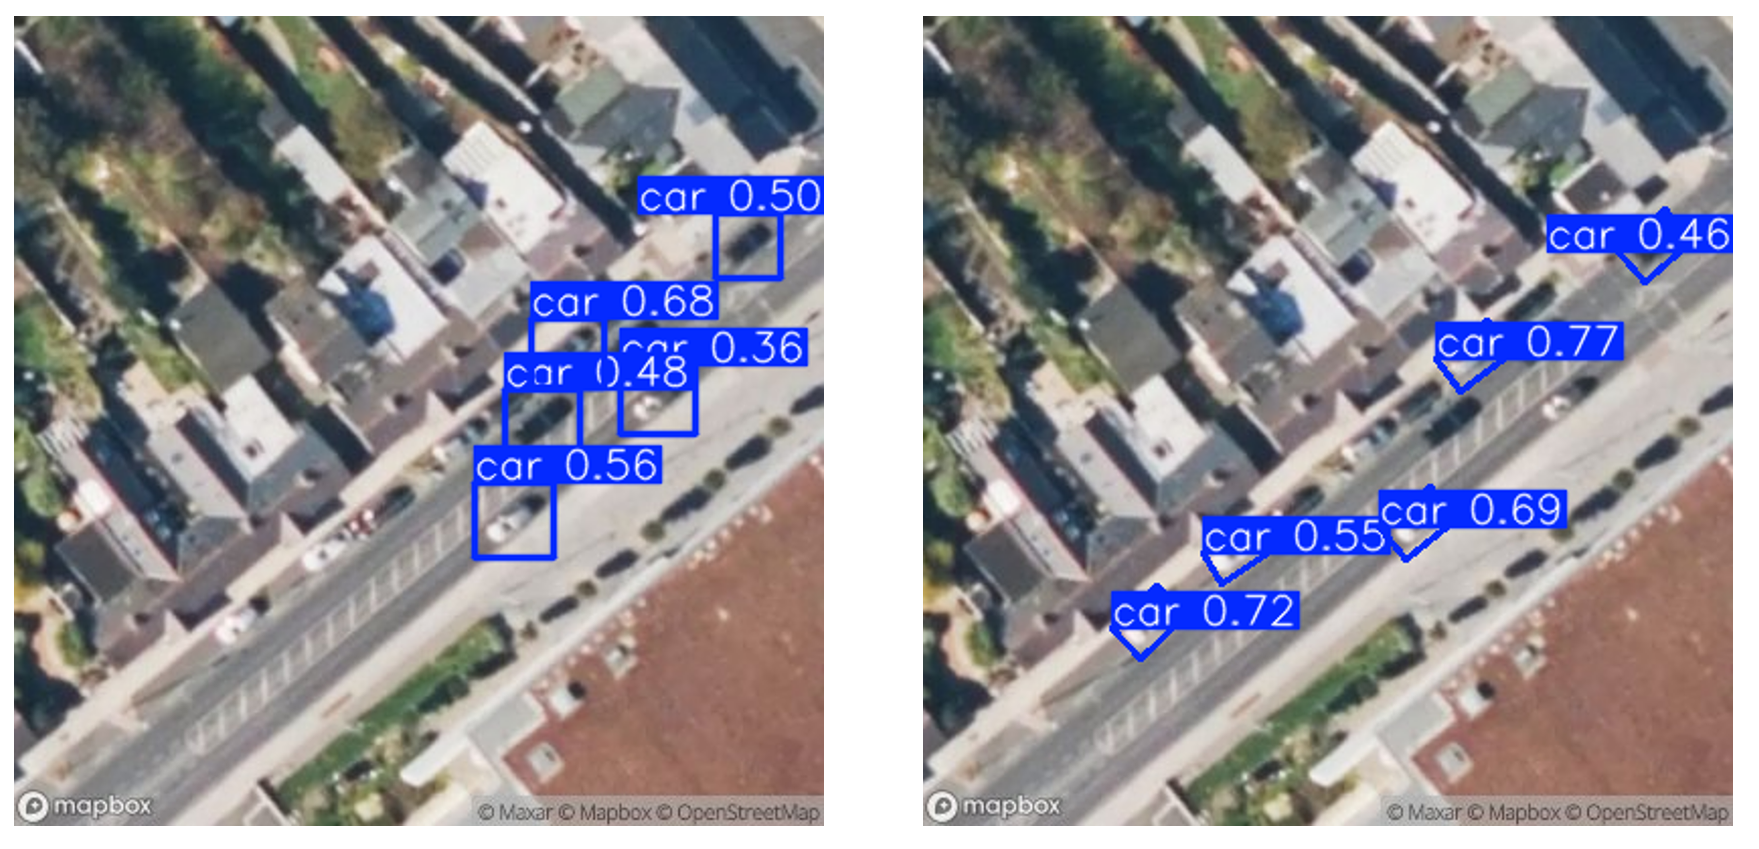
\includegraphics[width=0.85\textwidth]{images/obb-vs-nonobb-img.png}
  \caption{Non-OBB labels (left) versus OBB labels (right)}
\end{figure}
Thus, the YOLOv8-OBB model was trained on the settings below:
\begin{listing}[h!]
  \centering
  \begin{minted}{python3}
    train_results_obb = yolo8s_obb_model.train(data=data_config,
                  epochs=35,
                  patience=15,
                  optimizer="AdamW",    # Adam + weight decay for less overfitting
                  val=True, # validate during training
                  seed=1,
                  imgsz=416,
                  batch=16,
                  cache="disk",
                  )
  \end{minted}
\end{listing}
And the following results were obtained:
%yolov8 obb results
\begin{figure}[h!]
  \centering
  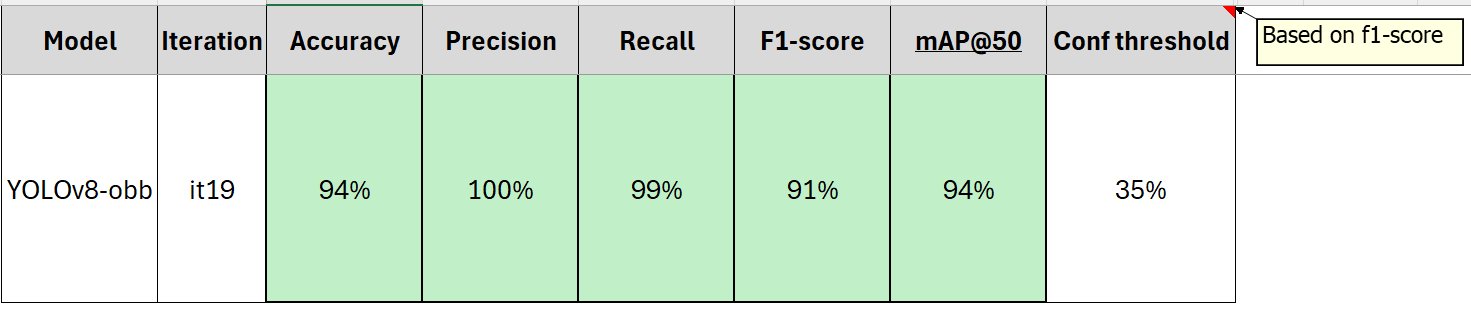
\includegraphics[width=0.85\textwidth]{images/yolo-obb-results.png}
  \caption{YOLOv8-OBB results}
\end{figure}

The weights were then obtained and used to identify cars in satellite images of the entire Dublin city using the script below.\\
\fcolorbox{yellow}{yellow}{Jess or Saul's script}

\subsubsection{Parking spot detection}
Subsequently, to identify the parking spots in each satellite image, the cars detected by the YOLO model are classified into on the road or parked, based on a road mask.

\subsubsection{Road mask generation}
Many different iterations of the road mask were used, the main iterations and their differences are explained and showed below.

The original mask was a very simple binary mask which identified the road pixels by their color, as the majority of roads were depicted in white and darkened the rest of the pixels in the image.

Through testing and thoroughly analysing the Mapbox Streets images, motorways and national roads were discovered to be depicted in yellow or orange. Therefore, two additional color masks (for orange and yellow) were concatenated to the original binary mask through bitwise operations.

To refine the mask, and reduce misclassification errors, additional annotations contained on the Mapbox Streets images such as street names and white dotted lines which denote a multitude of things (foot paths, planter boxes, pedestrian crosswalks, football fields delimitations, etc. ) were removed through morphological operations, leaving only a plain white line for each road.
A number of different kernel sizes, different contour thresholds and other parameters were tested to achieve the optimal removal of the street names and additional annotations.

A different approach using Canny Edge Detection was tested, however due to the nature of the Mapbox Streets images, the edges picked up were not significant and the overall performances was much worse than the current mask at the time.

A final improvement to the mask was made to avoid certain misclassification due to the Mapbox Streets road width not correctly reflecting all the lanes of the road and therefore classifying on the road cars as parked. This issue was most prominent for motorways and national roads and was resolved by enlarging those roads using a dilation technique. Multiple different kernel sizes, different number of iterations and kernels of different sizes applied consecutively were tested to find the optimal solution.

\subsubsection{Classifiction of cars into on the road or parked}
The cars detected by the Yolo model are then sorted into on the road or parked based on the road mask previously generated, which is explained in more detail below.

The model's predictions which are lower than the confidence threshold of 0.4 are discarded as they are more likely to be misclassifications, such as chimneys which were often misclassified as cars.

A bounding box for each of the model's predictions is computed from the center pixel coordinates, the width and the height returned from the model.
The overlap between the bounding box and the road pixels is calculated, and if the overlap is higher than the threshold of 0.5, the prediction is discarded, keeping only the parked cars.
Different thresholds were tested as well, however overall a harsher threshold works better given that these detections are used later on for the empty parking detection.

For each of the model's predictions for parked cars, the center pixels coordinates are mapped to geographic coordinates (longitude and latitude), and the width, height, rotation and orientation based on the angle are saved.

For testing and debugging purposes, all the bounding boxes of the cars found by the model are drawn onto the satellite image, on the road cars are drawn in blue while parked cars are drawn in red as seen in Figure ...

\subsubsection{Empty parking spot detection}
Subsequently, empty parking spots are detected between parked cars in each image, based on the parked cars detected by the Yolo model and classified using the road mask.
Originally 4 cases were considered, cars parked horizontally in a row or in a column, cars parked vertically in a column and parked vertically side by side. However horizontally parked in a column and vertically parked side by side were removed as they lead to too many misclassifications, namely the vertically parked side by side lead to adding many additional cars in driveways in residential areas.
A number of different variations and calculation techniques were tested out, however only the final version will be explained below.

Average parking spot width and length in pixels are calculated for each image, to draw the empty spots more uniformly. Average parking spot width and length in meters are set to 3.05 as found to be the optimal value through testing accounting for the variations in size.
Setting this value avoids misclassifications as previously the average width and length in meters were calculated dynamically, however in cases where the averages were lesser than 3, spots tended to overlap.

The parked cars detected are then sorted by latitude for horizontally aligned cars and by longitude for vertically aligned cars, to identify gaps between consecutive cars.
For each pair of consecutive spots, the distance in meters in between them is calculated. The gap is adjusted to account for the half cars on both sides, as the coordinates of the parked car represent the center of the car.
For the gaps smaller than the maximum gap threshold of 12 meters and larger than the average size of a car, where there is enough space to fit 1 or more car, and where the angle deviation is smaller than a threshold of 35 degrees, to ensure the spots are sufficiently aligned, the number of cars that fit into the gap is calculated.
Based on the number of empty spots found, the coordinates for those empty spots are calculated to be aligned with the 2 consecutive cars and then added to a list of empty spots detected.

Afterwards, duplicate spots defined as spots that overlap too much and where the distance between 2 spots is smaller than a threshold of 1 meter are removed.
As well, spots coinciding with cars identified by the Yolo model, where the distance between them is smaller than 1.25 meters are removed from the empty spots found.
Subsequently, empty spots that overlap with the road are filter out in a similar manner to the classification done by the road mask.

Following the detection of all the empty spots, the bounding boxes corresponding to each spot are drawn onto the satellite image in green.

\subsubsection{Classification of all spots detected}
All the parking spots detected, including the parked cars identified by the model and the empty parking spots are then classified into 3 different classes: public (on the street parking), private (residential parking) and parking lot, based on their proximity to the nearest road.

Multiple different clustering approaches were tested out to cluster spots together, such as DBSCAN, HDBSCAN and OPTICS.
Overall DBSCAN performed the best and the quickest out of all the clustering algorithms, given that some images contained very few parking spots, meaning clustering was only significant in cases with a minimum number of parking spots.
Through testing, the optimal hyperparmeters found for DBSCAN are \texttt{eps} : 55 and \texttt{min\_samples} : 5, which allow the correct identification of the clusters, avoiding misclassifications of residential areas with many cars as parking lots, which was a common misclassification initially, when the hyperparameters and thresholds were not set correctly.
\texttt{eps} refers to the maximum distance between two points for them to be considered as neighbors and \texttt{min\_samples} refers to the minimum number of points required to form a cluster.
HDBSCAN and OPTICS require a minimum number of samples larger or equal to 2, however given that not all images might contained at least 2 detections, clustering using those algorithms is not possible in all cases, so -1 is assigned to the spots without clusters which is the default behaviour of DBSCAN.
HDBSCAN gave similar results to DBSCAN, though not as good, while OPTICS only found smaller clusters which were not as significant.

Parking spots are classified as public if the proximity to the nearest road is less than a pixel threshold of 30, otherwise the parking spots are considered private. This optimal threshold was found through extensive testing on a test set containing various edge cases.
Parking spots are classified as parking lots, when clusters of 18 or more spots are identified in an image. Larger clusters are prioritized as parking lots containing less spots are not as relevant to the target user and given that the threshold of 18 spots minimizes the risk of misclassifying residential areas as parking lots.

Afterwards, clusters and classification labels are drawn onto the satellite image. The clusters are color coded and denoted as a circle at the center of the bounding box, while the classification label is written to the right of the bounding box. The private in written in red, public in green and parking lot in white.

\subsubsection{Uploading points to the backend server}
The longitude, latitude and classification of all the parking spots detected are then saved to a csv file.
Potential spot duplicates are dropped, as the same car may be in multiple images given that the images are defined by their center coordinates, which causes adjacent images to overlap and share common areas. (The rightmost part of one image often overlaps with the leftmost part of another image.)

Subsequently, the parking zones and costs associated to each parking spot found are added to the csv file.
Dublin defines different parking zones by color, based on their high to moderate demand which changes the price per zone as seen below in Figure ...

The csv file containing the longitude, latitude, classification label, parking zone and parking cost is then uploaded to the PostgreSQL database, in the backend server using the \texttt{send\_points.py} script.

\subsubsection{Evaluation of each submodule of the parking detection model}
Each major section of the parking detection model was evaluated individually in order to access the overall performance. The results will be presented and analysed for each section below.

\subsubsection{Evaluation of the Yolo model}

\subsubsection{Evaluation of the classifiction of cars into on the road or parked}
The classification of cars into on the road or parked by the road mask is evaluated in the \texttt{evaluate\_road\_mask.py} Python script.
The classification is evaluated on the following metrics: Average Intersection over Union (IoU), Balanced Accuracy and Precision, Recall, F1 Score, Accuracy, Specificity per class. These metrics are saved in a csv file for each test image as well as the overall average metrics on the entire test set.

A test set of 50 images was carefully selected to include edge cases and difficult cases and then consistently labelled in the labelling software Label Studio. The labels are drawn without rotation to ensure the maximum overlap, as the labels are exported to \texttt{txt} format and include only the pixel coordinates, width and  height of the bounding boxes annotated.

The overall results on test set are presented below in Table~\ref{tab:metrics1}

\begin{table}[h]
  \centering
  \begin{tabular}{|l|c|c|}
    \hline
    \textbf{Metric}           & \textbf{Parked} & \textbf{Road} \\ \hline
    Average IoU               & 0.66            & 0.66          \\ \hline
    Average Balanced Accuracy & 0.58            & 0.58          \\ \hline
    Average Precision         & 0.70            & 0.90          \\ \hline
    Average Recall            & 0.75            & 0.67          \\ \hline
    Average F1 Score          & 0.59            & 0.54          \\ \hline
    Average Accuracy          & 0.69            & 0.64          \\ \hline
    Average Specificity       & 0.74            & 0.79          \\ \hline
  \end{tabular}
  \caption{Performance Metrics for Road Mask Classification}
  \label{tab:metrics1}
\end{table}

Analyse metrics + Mention common problems. Reference similar results in object detection

Some images from the test set can be seen below, in Table~\ref{tab:test_images1}
The predicted parked cars are drawn in red while the true labels are drawn in light pink. The predicted on the road cars are drawn in blue while the true labels are drawn in cyan.

\begin{table}[h]
  \centering
  \begin{tabular}{cc}
    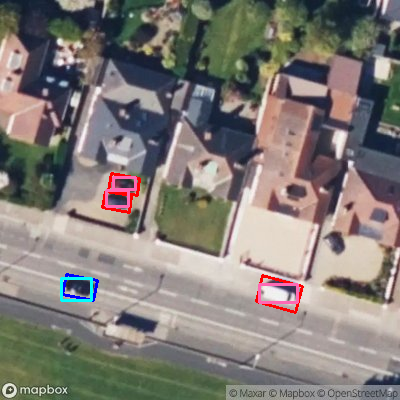
\includegraphics[width=0.4\textwidth]{images/image1_road_mask_classification_test_set.png} & 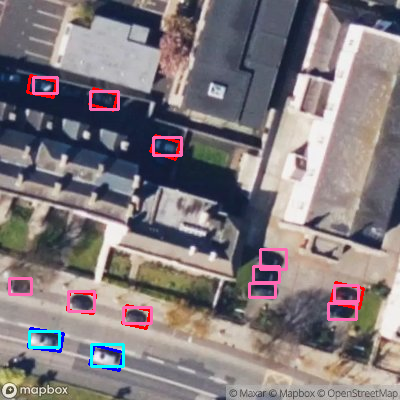
\includegraphics[width=0.4\textwidth]{images/image2_road_mask_classification_test_set.png} \\
    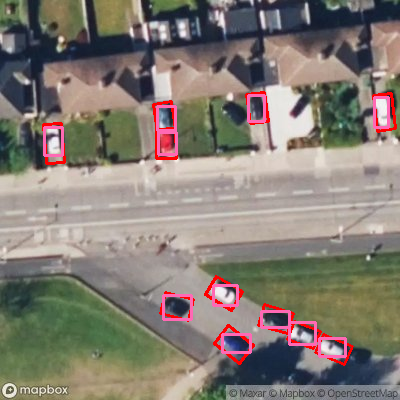
\includegraphics[width=0.4\textwidth]{images/image3_road_mask_classification_test_set.png} & 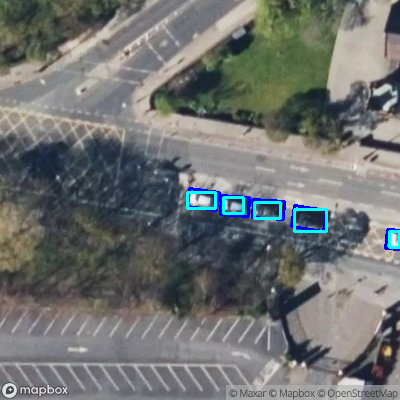
\includegraphics[width=0.4\textwidth]{images/image4_road_mask_classification_test_set.png} \\
    \multicolumn{2}{c}{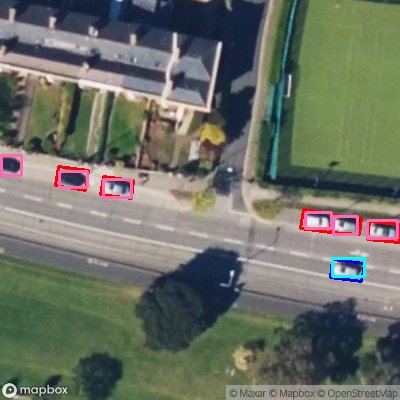
\includegraphics[width=0.4\textwidth]{images/image5_road_mask_classification_test_set.png}}                                                                          \\
  \end{tabular}
  \caption{Images from the Road Mask Classification Test Set}
  \label{tab:test_images1}
\end{table}

\subsubsection{Evaluation of the empty parking detection}
The empty parking detection logic is evaluated in the \texttt{evaluate\_empty\_parking\_detection.py} Python script.
Expliquer script, comment l'orientation est calcule de facon automatique.
The classification is evaluated on the following metrics: Average IoU, Average Precision, Average Recall, Average F1 Score, Average Orientation Accuracy, Average Spot Detection Ratio (SDR), Average Spot Detection Error (SDE), Average False Positive Rate (FPR), and Average False Negative Rate (FNR).
Explain metrics and how the additional ones are calculated/ what they represent.
These metrics are then saved in a csv file for each test image as well as the overall average metrics on the entire test set.

Likewise a test set of 50 images was carefully selected and consistently labelled in Label Studio, without rotation to ensure the maximum overlap.
Achieving a high IoU was a significant challenge, specifically in this section, as the positioning of the spots can be difficult to label.
To remedy this issue, the IoU threshold was lowered to 0.35, as there was still significant overlap visible when analysing the test images.
The problems linked to overlap, is equally due to the differences in orientation as the true labels and the predictions are not calculated in a similar manner. (Expliquer mieux et dire les differences)

The overall results on test set are presented below in Table~\ref{tab:metrics2}

\begin{table}[h]
  \centering
  \begin{tabular}{|l|c|}
    \hline
    \textbf{Metric}                    & \textbf{Value} \\ \hline
    Average IoU                        & 0.59           \\ \hline
    Average Precision                  & 0.77           \\ \hline
    Average Recall                     & 0.70           \\ \hline
    Average F1 Score                   & 0.69           \\ \hline
    Average Orientation Accuracy       & 0.64           \\ \hline
    Average Spot Detection Ratio (SDR) & 1.05           \\ \hline
    Average Spot Detection Error (SDE) & 1.44           \\ \hline
    Average False Positive Rate (FPR)  & 0.23           \\ \hline
    Average False Negative Rate (FNR)  & 0.22           \\ \hline
  \end{tabular}
  \caption{Performance Metrics for Empty Parking Detection}
  \label{tab:metrics2}
\end{table}

Analyse metrics + Mention common problems. Reference similar results in object detection

A few images from the test set are displayed below, in Table~\ref{tab:test_images2}
The predicted empty parking spots are drawn in green while the true labels are in light pink.

\begin{table}[h]
  \centering
  \begin{tabular}{cc}
    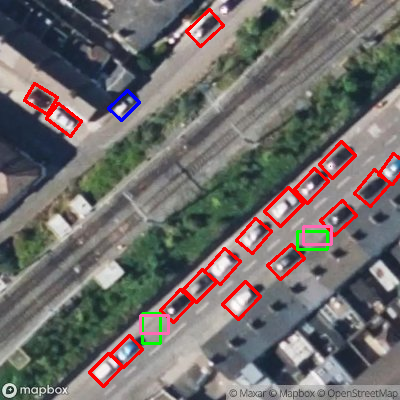
\includegraphics[width=0.4\textwidth]{images/image1_empty_parking_detection_test_set.png} & 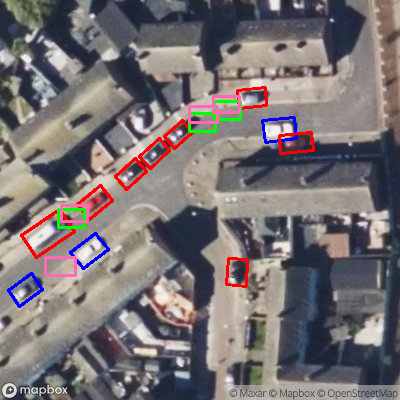
\includegraphics[width=0.4\textwidth]{images/image2_empty_parking_detection_test_set.png} \\
    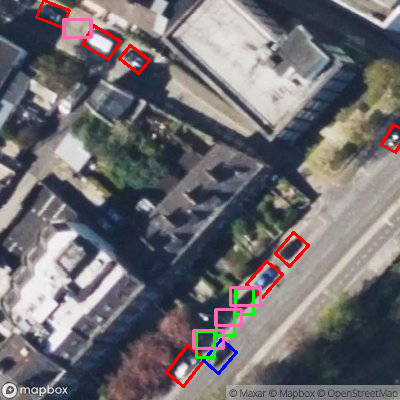
\includegraphics[width=0.4\textwidth]{images/image3_empty_parking_detection_test_set.png} & 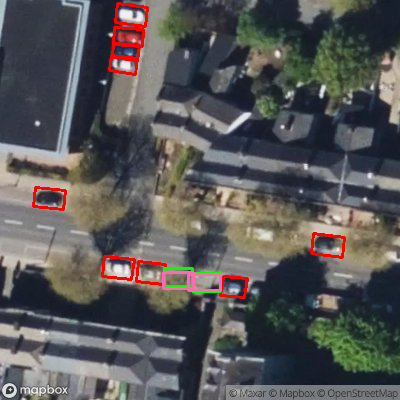
\includegraphics[width=0.4\textwidth]{images/image4_empty_parking_detection_test_set.png} \\
    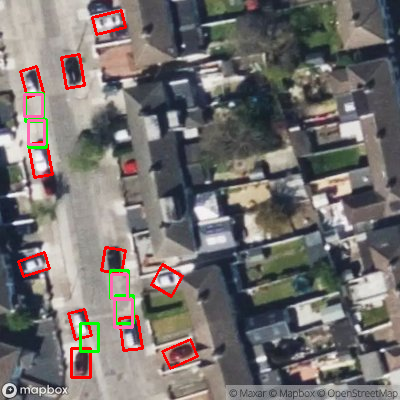
\includegraphics[width=0.4\textwidth]{images/image5_empty_parking_detection_test_set.png} & 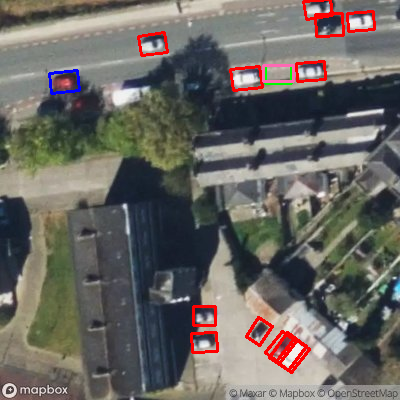
\includegraphics[width=0.4\textwidth]{images/image6_empty_parking_detection_test_set.png} \\
  \end{tabular}
  \caption{Images from the Empty Parking Detection Test Set}
  \label{tab:test_images2}
\end{table}

\subsubsection{Evaluation of the classification of the spots detected into private, public and parking lot}
The classification of the spots detected into private, public and parking lot is evaluated in the \texttt{evaluate\_classification\_of\_spots.py} Python script.
Dire changement, like all the spots include everything...
The classification is evaluated on the following metrics: Average IoU, Balanced Accuracy and Precision, Recall, F1 Score, Accuracy, Specificity per class. These metrics are saved in a csv file for each test image as well as the overall average metrics on the entire test set.

Similarly, a test set of 50 images was carefully selected and consistently labelled in Label Studio, without rotation to ensure the maximum overlap.

The overall results on test set are presented below in Table~\ref{tab:metrics3}

\begin{table}[h]
  \centering
  \begin{tabular}{|l|c|c|c|}
    \hline
    \textbf{Metric}           & \textbf{Public} & \textbf{Private} & \textbf{Parking Lot} \\ \hline
    Average IoU               & 0.60            & 0.60             & 0.60                 \\ \hline
    Average Balanced Accuracy & 0.57            & 0.57             & 0.57                 \\ \hline
    Average Precision         & 0.73            & 0.65             & 0.59                 \\ \hline
    Average Recall            & 0.72            & 0.75             & 0.74                 \\ \hline
    Average F1 Score          & 0.68            & 0.62             & 0.61                 \\ \hline
    Average Accuracy          & 0.67            & 0.54             & 0.63                 \\ \hline
    Average Specificity       & 0.59            & 0.54             & 0.41                 \\ \hline
  \end{tabular}
  \caption{Performance Metrics for Parking Spot Classification}
  \label{tab:metrics3}
\end{table}

Analyse metrics + Mention common problems. Reference similar results in object detection

A few images from the test set are shown below, in Table~\ref{tab:test_images3}
The predicted public spots are drawn in green while the true labels are in dark green. The predicted private spots are highlighted in red while the true labels are in light pink. The predicted parking lot spots are shown in blue while the true labels are in cyan.

\begin{table}[h]
  \centering
  \begin{tabular}{cc}
    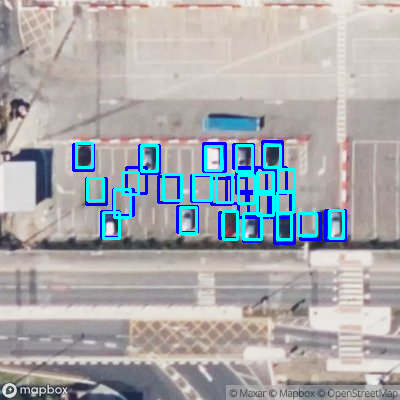
\includegraphics[width=0.4\textwidth]{images/image1_classification_test_set.png} & 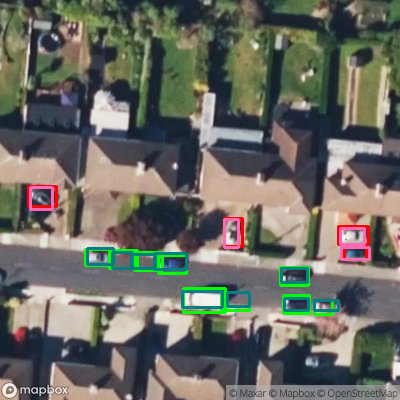
\includegraphics[width=0.4\textwidth]{images/image2_classification_test_set.png} \\
    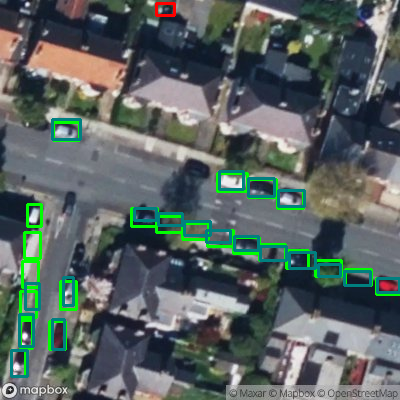
\includegraphics[width=0.4\textwidth]{images/image3_classification_test_set.png} & 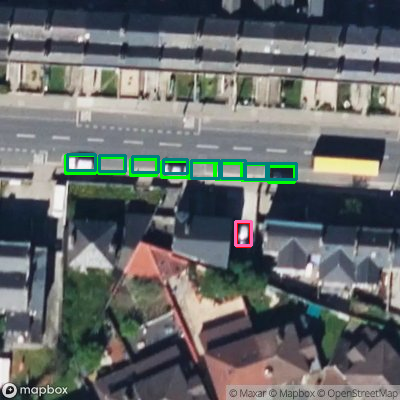
\includegraphics[width=0.4\textwidth]{images/image4_classification_test_set.png} \\
    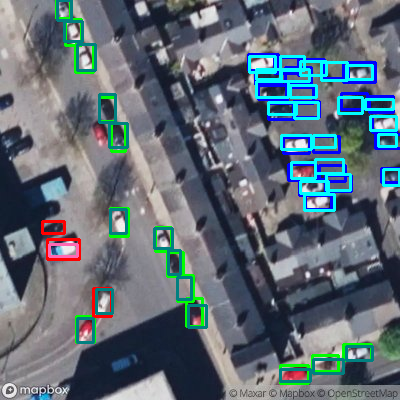
\includegraphics[width=0.4\textwidth]{images/image5_classification_test_set.png} & 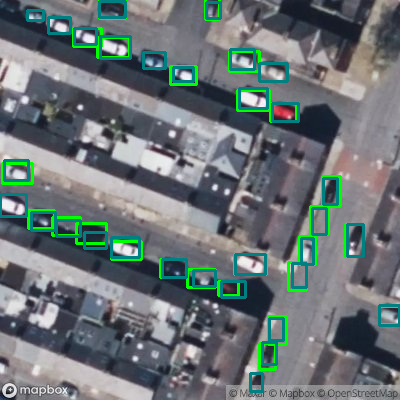
\includegraphics[width=0.4\textwidth]{images/image6_classification_test_set.png} \\
  \end{tabular}
  \caption{Images from the Parking Spot Classification Test Set}
  \label{tab:test_images3}
\end{table}


Relire tout and add more, ajouter totues les figures. Expliquer parking zones and costs mieux en ajoutant la figure du pdf.
Verifier que j'ai explique toutes les fonctions. Refer to each figures, like say as seen in figure x ...